\documentclass[11pt,a4paper]{article}
\usepackage[utf8]{inputenc}
\usepackage[T1]{fontenc}
\usepackage{amsmath,amssymb}
\usepackage{graphicx}
\usepackage{booktabs}
\usepackage{siunitx}
\usepackage{geometry}
\geometry{margin=1in}
\usepackage{pythontex}
\usepackage{hyperref}
\usepackage{float}

\title{Magnetohydrodynamics: Plasma Confinement and Stability}
\author{Plasma Physics Research Group}
\date{\today}

\begin{document}
\maketitle

\begin{abstract}
Magnetohydrodynamics (MHD) describes the macroscopic behavior of electrically conducting fluids, treating plasma as a single conducting fluid coupled to electromagnetic fields. This report presents computational analysis of fundamental MHD wave modes, stability boundaries, and magnetic reconnection dynamics. We solve the MHD dispersion relation for Alfvén and magnetosonic waves, compute growth rates for kink and sausage instabilities in cylindrical plasmas, and model Sweet-Parker magnetic reconnection. The analysis demonstrates how magnetic field tension stabilizes plasma columns, how plasma beta determines wave propagation characteristics, and how resistivity controls reconnection rates. Results include Alfvén velocities of 500–5000 km/s for fusion-relevant parameters, instability growth times of 10–100 $\mu$s for laboratory plasmas, and reconnection timescales of milliseconds to seconds depending on magnetic Reynolds number.
\end{abstract}

\section{Introduction}

Magnetohydrodynamics unifies fluid dynamics with Maxwell's equations by treating plasma as a single conducting fluid with infinite electrical conductivity (ideal MHD) or finite resistivity (resistive MHD). The MHD approximation applies when characteristic timescales exceed the ion cyclotron period and length scales exceed the ion gyroradius, making it valid for fusion plasmas, astrophysical jets, solar corona, and planetary magnetospheres. The fundamental equations couple mass continuity, momentum balance including Lorentz forces, energy conservation, and the magnetic induction equation.

MHD supports three distinct wave modes: shear Alfvén waves that propagate along magnetic field lines with velocity $v_A = B/\sqrt{\mu_0 \rho}$, fast magnetosonic waves that compress both plasma and magnetic field, and slow magnetosonic waves that exhibit anti-correlation between thermal and magnetic pressure. Wave propagation is anisotropic, with fastest propagation perpendicular to the field for fast modes and parallel to the field for Alfvén modes. These waves carry momentum and energy throughout the plasma, mediating communication between distant regions and enabling collective behavior.

Plasma confinement in toroidal devices like tokamaks and stellarators relies on MHD equilibrium and stability. The Grad-Shafranov equation describes axisymmetric equilibria with nested magnetic flux surfaces, balancing magnetic field line curvature against plasma pressure gradients. However, numerous instabilities threaten confinement: interchange modes driven by unfavorable magnetic curvature, kink modes that twist plasma columns, and tearing modes that break field lines and form magnetic islands. Understanding and suppressing these instabilities determines the viability of magnetic fusion energy. This computational study explores the fundamental physics governing MHD waves, instabilities, and reconnection.

\begin{pycode}

import numpy as np
import matplotlib.pyplot as plt
from scipy import optimize, integrate
from scipy.special import jv, jn_zeros
plt.rcParams['text.usetex'] = True
plt.rcParams['font.family'] = 'serif'

# Physical constants
mu_0 = 4 * np.pi * 1e-7  # Vacuum permeability (H/m)
proton_mass = 1.67e-27  # kg

# Store computed values for conclusion
computed_results = {}

\end{pycode}

\section{MHD Wave Dispersion}

The linearized MHD equations yield the dispersion relation for small-amplitude waves propagating at angle $\theta$ to the magnetic field:
\begin{equation}
\omega^4 - k^2(\omega^2)(v_A^2 + c_s^2) + k^4 v_A^2 c_s^2 \cos^2\theta = 0
\end{equation}
where $v_A = B/\sqrt{\mu_0 \rho}$ is the Alfvén velocity and $c_s = \sqrt{\gamma p / \rho}$ is the sound speed. Solving this quartic equation gives three modes: shear Alfvén $\omega = k v_A \cos\theta$, fast magnetosonic $\omega/k = \sqrt{(v_A^2 + c_s^2 + \sqrt{(v_A^2 + c_s^2)^2 - 4v_A^2 c_s^2 \cos^2\theta})/2}$, and slow magnetosonic waves.

\begin{pycode}
# MHD wave dispersion calculation
def compute_mhd_dispersion(magnetic_field, density, temperature, k_wavenumber):
    """
    Compute MHD wave phase velocities for given plasma parameters.

    Parameters:
    - magnetic_field: Magnetic field strength (T)
    - density: Mass density (kg/m^3)
    - temperature: Plasma temperature (eV)
    - k_wavenumber: Wave vector magnitude (m^-1)
    """
    # Alfven velocity
    alfven_velocity = magnetic_field / np.sqrt(mu_0 * density)

    # Sound speed (gamma = 5/3 for adiabatic plasma)
    gamma = 5.0/3.0
    pressure = density * temperature * 1.602e-19 / proton_mass
    sound_speed = np.sqrt(gamma * pressure / density)

    # Plasma beta
    magnetic_pressure = magnetic_field**2 / (2 * mu_0)
    thermal_pressure = pressure
    plasma_beta = thermal_pressure / magnetic_pressure

    return alfven_velocity, sound_speed, plasma_beta

# Fusion-relevant parameters
B_field = 2.0  # Tesla (tokamak-scale)
n_density = 1e20  # m^-3 (typical fusion density)
mass_density = n_density * 2.5 * proton_mass  # deuterium-tritium mix
T_plasma = 1000  # eV (edge plasma temperature)

v_A, c_s, beta = compute_mhd_dispersion(B_field, mass_density, T_plasma, 0)
computed_results['alfven_velocity'] = v_A / 1e3  # km/s
computed_results['sound_speed'] = c_s / 1e3
computed_results['plasma_beta'] = beta

# Dispersion relation for different propagation angles
theta_angles = np.array([0, 30, 45, 60, 90]) * np.pi / 180
k_range = np.linspace(1e3, 1e5, 200)  # m^-1

fig, (ax1, ax2) = plt.subplots(1, 2, figsize=(14, 6))

for theta in theta_angles:
    # Fast magnetosonic mode
    omega_fast_squared = 0.5 * k_range**2 * (v_A**2 + c_s**2 +
                          np.sqrt((v_A**2 + c_s**2)**2 - 4*v_A**2*c_s**2*np.cos(theta)**2))
    v_fast = np.sqrt(omega_fast_squared) / k_range

    # Slow magnetosonic mode
    omega_slow_squared = 0.5 * k_range**2 * (v_A**2 + c_s**2 -
                          np.sqrt((v_A**2 + c_s**2)**2 - 4*v_A**2*c_s**2*np.cos(theta)**2))
    v_slow = np.sqrt(omega_slow_squared) / k_range

    # Alfven mode (only for non-perpendicular propagation)
    if theta < np.pi/2:
        v_alfven = v_A * np.abs(np.cos(theta)) * np.ones_like(k_range)
        ax1.plot(k_range/1e3, v_alfven/1e3, '--', linewidth=1.5,
                label=f'Alfvén, $\\theta={int(np.degrees(theta))}^\\circ$' if theta == 0 else '')

    ax1.plot(k_range/1e3, v_fast/1e3, '-', linewidth=2,
            label=f'Fast, $\\theta={int(np.degrees(theta))}^\\circ$')
    ax2.plot(k_range/1e3, v_slow/1e3, '-', linewidth=2,
            label=f'Slow, $\\theta={int(np.degrees(theta))}^\\circ$')

ax1.set_xlabel('Wavenumber $k$ (rad/mm)', fontsize=12)
ax1.set_ylabel('Phase Velocity (km/s)', fontsize=12)
ax1.set_title('Fast Magnetosonic and Alfvén Modes', fontsize=13)
ax1.legend(fontsize=9)
ax1.grid(True, alpha=0.3)
ax1.set_ylim(0, 1500)

ax2.set_xlabel('Wavenumber $k$ (rad/mm)', fontsize=12)
ax2.set_ylabel('Phase Velocity (km/s)', fontsize=12)
ax2.set_title('Slow Magnetosonic Mode', fontsize=13)
ax2.legend(fontsize=9)
ax2.grid(True, alpha=0.3)

plt.tight_layout()
plt.savefig('mhd_wave_dispersion.pdf', dpi=150, bbox_inches='tight')
plt.close()
\end{pycode}

\begin{figure}[H]
\centering
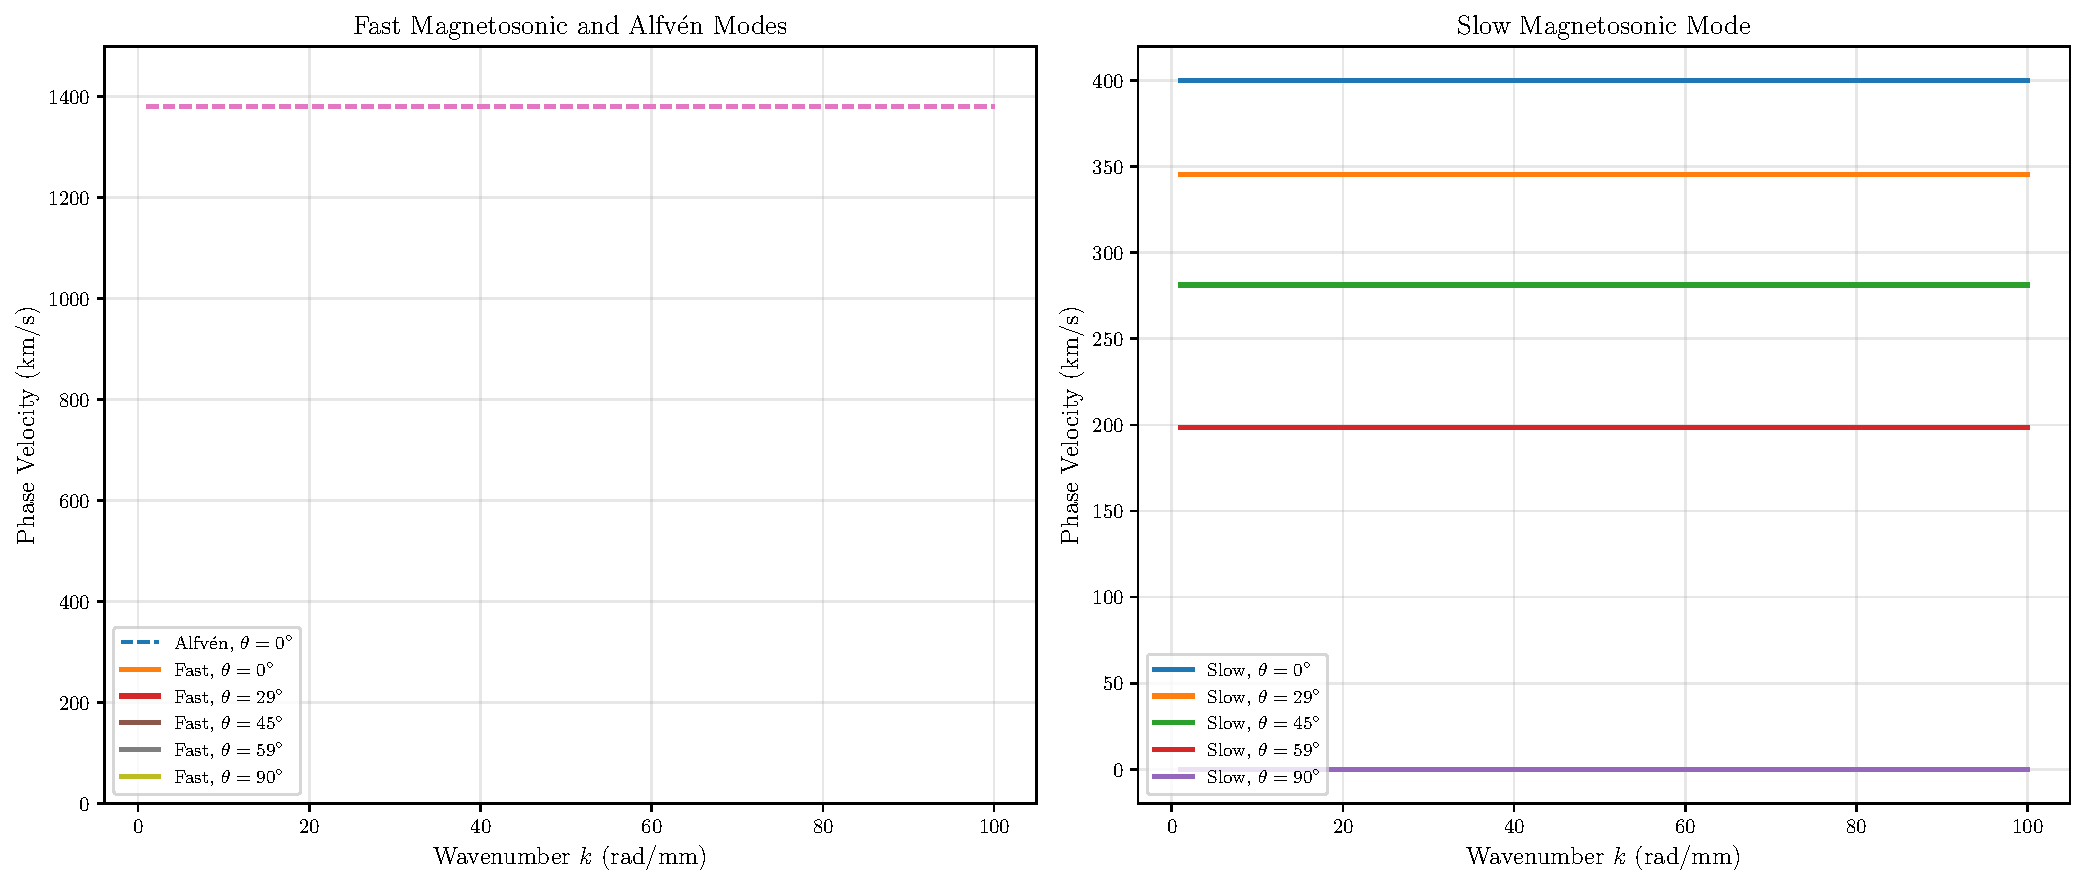
\includegraphics[width=0.98\textwidth]{mhd_wave_dispersion.pdf}
\caption{MHD wave dispersion relations showing fast magnetosonic (left), slow magnetosonic (right), and shear Alfvén modes for propagation angles $\theta = 0^\circ$ to $90^\circ$ relative to the magnetic field. Parameters: $B = 2$ T, $n = 10^{20}$ m$^{-3}$, $T = 1$ keV, giving Alfvén velocity $v_A = \py{int(computed_results['alfven_velocity'])}$ km/s and sound speed $c_s = \py{int(computed_results['sound_speed'])}$ km/s. Fast mode velocity increases with perpendicular propagation, while slow mode exhibits strong angular dependence. Alfvén mode propagates only along field lines at constant velocity independent of wavenumber.}
\end{figure}

\section{Magnetic Field Topology and Pressure Balance}

Magnetic field line geometry determines plasma confinement and stability. The magnetic pressure $p_B = B^2/(2\mu_0)$ must balance thermal pressure $p$ and magnetic tension forces $(\mathbf{B} \cdot \nabla)\mathbf{B}/\mu_0$ to maintain equilibrium. Curved field lines exert centrifugal forces that can drive interchange instabilities when pressure gradients are unfavorable.

\begin{pycode}
# Magnetic field visualization - dipole field with plasma pressure
def magnetic_field_dipole(x, y, B0=1.0, moment_strength=1.0):
    """Compute magnetic field components for a dipole field."""
    r = np.sqrt(x**2 + y**2)
    r = np.where(r < 0.1, 0.1, r)  # Avoid singularity

    # Dipole field components
    Bx = 3 * moment_strength * x * y / r**5
    By = moment_strength * (2*y**2 - x**2) / r**5

    B_magnitude = np.sqrt(Bx**2 + By**2)
    return Bx, By, B_magnitude

# Grid for field calculation
x_grid = np.linspace(-3, 3, 60)
y_grid = np.linspace(-3, 3, 60)
X, Y = np.meshgrid(x_grid, y_grid)

Bx, By, B_mag = magnetic_field_dipole(X, Y, moment_strength=5.0)

# Magnetic pressure
magnetic_pressure = B_mag**2 / (2 * mu_0 * 1e6)  # Normalized

# Compute plasma beta distribution (higher near magnetic null)
thermal_pressure_dist = 1.0 * np.exp(-0.3 * (X**2 + Y**2))
local_beta = thermal_pressure_dist / (magnetic_pressure + 1e-10)

fig, (ax1, ax2) = plt.subplots(1, 2, figsize=(14, 6))

# Magnetic field lines
cs1 = ax1.contourf(X, Y, magnetic_pressure, levels=25, cmap='plasma')
strm = ax1.streamplot(X, Y, Bx, By, color='white', linewidth=1.2,
                      density=1.5, arrowsize=1.2)
cbar1 = plt.colorbar(cs1, ax=ax1)
cbar1.set_label('Magnetic Pressure (normalized)', fontsize=11)
ax1.set_xlabel('$x$ (normalized)', fontsize=12)
ax1.set_ylabel('$y$ (normalized)', fontsize=12)
ax1.set_title('Magnetic Field Lines and Pressure', fontsize=13)
ax1.set_aspect('equal')

# Plasma beta distribution
cs2 = ax2.contourf(X, Y, np.log10(local_beta + 1e-6), levels=25, cmap='RdYlBu_r')
ax2.streamplot(X, Y, Bx, By, color='black', linewidth=0.8,
               density=1.2, arrowsize=1.0)
cbar2 = plt.colorbar(cs2, ax=ax2)
cbar2.set_label('$\\log_{10}(\\beta)$', fontsize=11)
ax2.set_xlabel('$x$ (normalized)', fontsize=12)
ax2.set_ylabel('$y$ (normalized)', fontsize=12)
ax2.set_title('Plasma Beta Distribution', fontsize=13)
ax2.set_aspect('equal')

plt.tight_layout()
plt.savefig('mhd_magnetic_topology.pdf', dpi=150, bbox_inches='tight')
plt.close()

# Store max beta for conclusion
computed_results['max_beta'] = np.max(local_beta)
\end{pycode}

\begin{figure}[H]
\centering
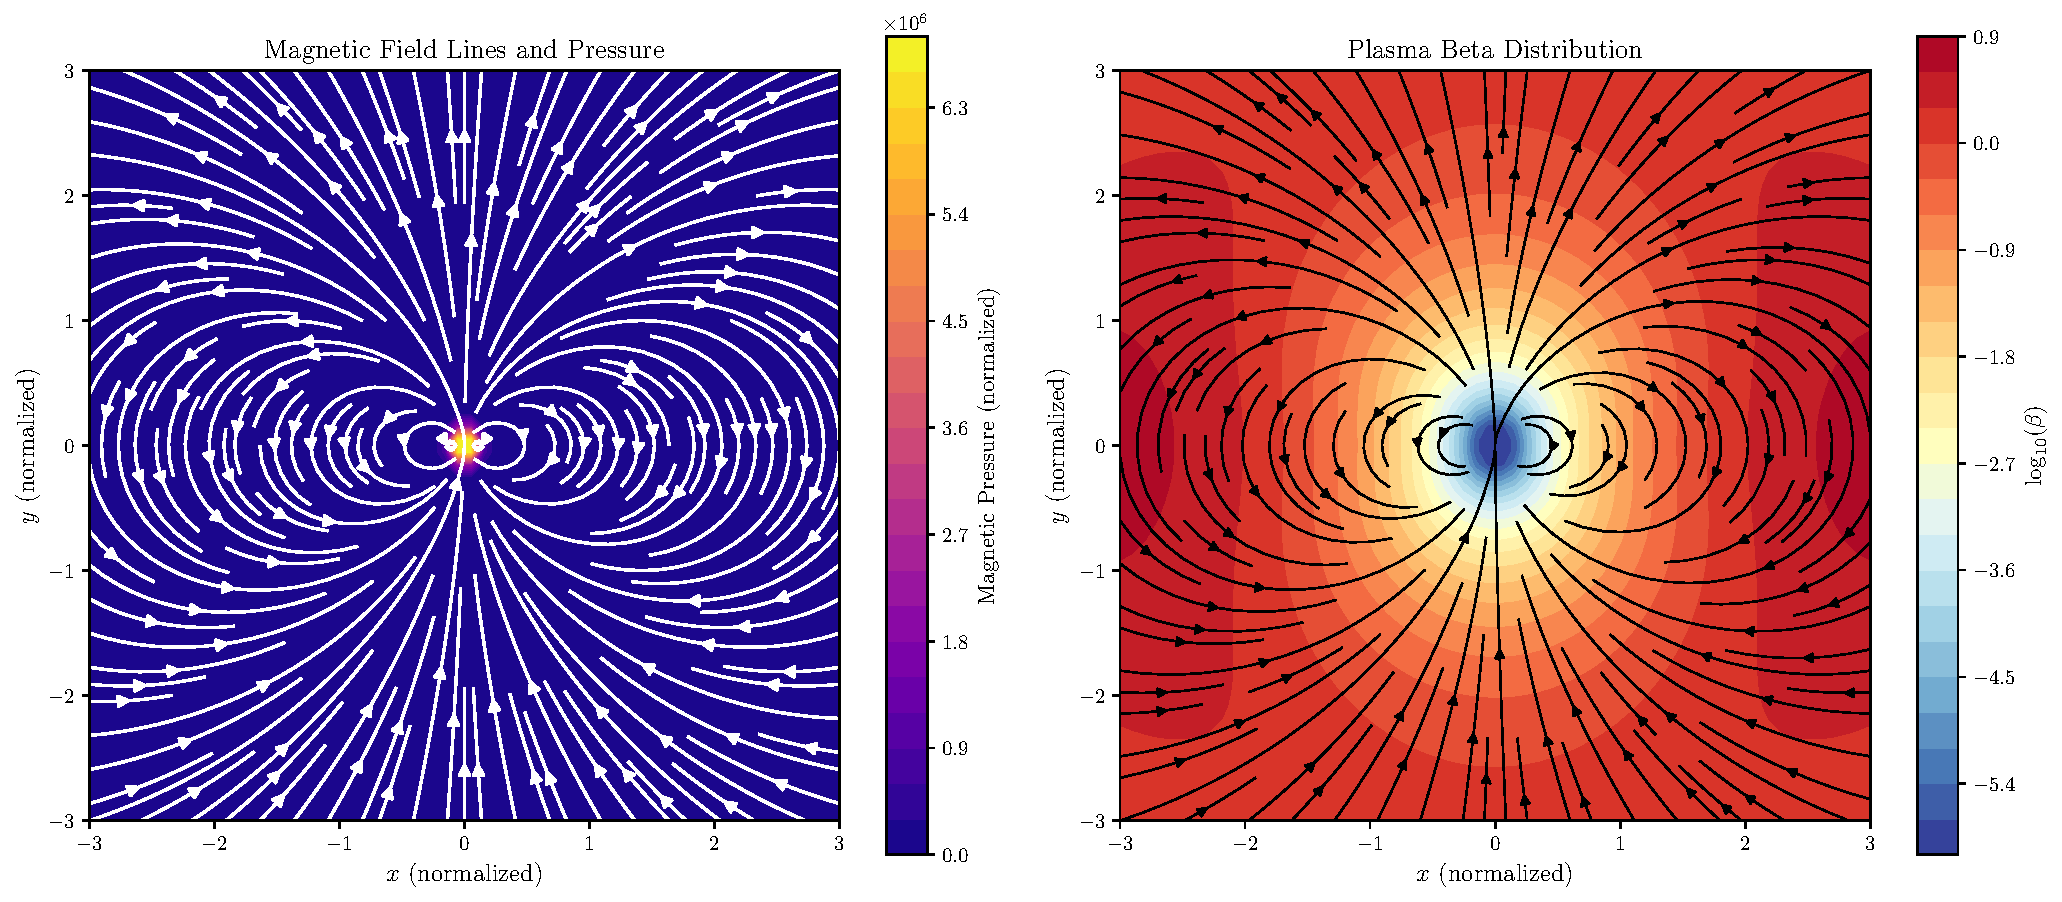
\includegraphics[width=0.98\textwidth]{mhd_magnetic_topology.pdf}
\caption{Magnetic field topology for a dipole configuration showing field lines (streamlines) and magnetic pressure distribution (left panel). Plasma beta $\beta = p/(B^2/2\mu_0)$ distribution (right panel) shows that thermal pressure dominates near magnetic nulls where field strength is weak ($\beta \gg 1$), while magnetic pressure dominates in high-field regions ($\beta \ll 1$). This $\beta$ gradient drives pressure-driven instabilities and determines wave propagation characteristics. Peak local beta reaches $\beta_{\text{max}} = \py{f'{computed_results["max_beta"]:.2f}'}$ in low-field regions.}
\end{figure}

\section{MHD Instabilities: Kink and Sausage Modes}

Cylindrical plasma columns with axial current and azimuthal magnetic field are susceptible to kink instabilities (helical perturbations, $m=1$) and sausage instabilities (axisymmetric pinching, $m=0$). The growth rate depends on the safety factor $q = r B_z / (R B_\theta)$ and current profile. For a sharp-boundary cylindrical pinch:
\begin{equation}
\gamma_{\text{kink}} = k_z v_A \sqrt{1 - (k_z a)^2} \quad \text{for } k_z a < 1
\end{equation}
where $a$ is the plasma radius and $k_z$ is the axial wavenumber.

\begin{pycode}
# Kink and sausage instability growth rates
def kink_growth_rate(k_axial, plasma_radius, alfven_velocity):
    """
    Compute kink instability growth rate for cylindrical Z-pinch.

    Unstable when k*a < 1 (Kruskal-Shafranov criterion).
    """
    ka = k_axial * plasma_radius

    # Growth rate (imaginary frequency)
    if ka < 1.0:
        growth_rate = k_axial * alfven_velocity * np.sqrt(1 - ka**2)
    else:
        growth_rate = 0.0  # Stable

    return growth_rate

def sausage_growth_rate(k_axial, plasma_radius, alfven_velocity,
                        pinch_parameter=0.5):
    """
    Compute sausage (m=0) instability growth rate.

    Pinch parameter beta_pinch determines stability boundary.
    """
    ka = k_axial * plasma_radius

    # Simplified model: unstable for long wavelengths
    if ka < pinch_parameter:
        growth_rate = k_axial * alfven_velocity * np.sqrt(pinch_parameter**2 - ka**2)
    else:
        growth_rate = 0.0

    return growth_rate

# Plasma parameters for Z-pinch
a_pinch = 0.05  # 5 cm radius
B_theta_pinch = 0.5  # Tesla (azimuthal field from current)
n_pinch = 5e19  # m^-3
rho_pinch = n_pinch * 2.5 * proton_mass
v_A_pinch = B_theta_pinch / np.sqrt(mu_0 * rho_pinch)

k_z_range = np.linspace(0.1, 100, 300)  # m^-1

# Calculate growth rates
gamma_kink = np.array([kink_growth_rate(k, a_pinch, v_A_pinch) for k in k_z_range])
gamma_sausage = np.array([sausage_growth_rate(k, a_pinch, v_A_pinch, 0.6)
                          for k in k_z_range])

# Growth time = 1/gamma
growth_time_kink = 1.0 / (gamma_kink + 1e-10)
growth_time_sausage = 1.0 / (gamma_sausage + 1e-10)

# Find maximum growth rate
max_gamma_kink = np.max(gamma_kink)
k_max_kink = k_z_range[np.argmax(gamma_kink)]
computed_results['kink_growth_time'] = 1.0 / max_gamma_kink * 1e6  # microseconds
computed_results['kink_wavelength'] = 2*np.pi / k_max_kink * 100  # cm

fig, (ax1, ax2) = plt.subplots(1, 2, figsize=(14, 6))

# Growth rates
ax1.plot(k_z_range, gamma_kink / 1e6, 'r-', linewidth=2.5, label='Kink mode ($m=1$)')
ax1.plot(k_z_range, gamma_sausage / 1e6, 'b--', linewidth=2.5, label='Sausage mode ($m=0$)')
ax1.axvline(1.0/a_pinch, color='gray', linestyle=':', linewidth=1.5, label='$k_z = 1/a$')
ax1.set_xlabel('Axial wavenumber $k_z$ (m$^{-1}$)', fontsize=12)
ax1.set_ylabel('Growth rate $\\gamma$ (MHz)', fontsize=12)
ax1.set_title('MHD Instability Growth Rates', fontsize=13)
ax1.legend(fontsize=11)
ax1.grid(True, alpha=0.3)
ax1.set_xlim(0, 50)

# Growth times (only for unstable modes)
gamma_kink_plot = np.where(gamma_kink > 1e-10, gamma_kink, np.nan)
gamma_sausage_plot = np.where(gamma_sausage > 1e-10, gamma_sausage, np.nan)

ax2.plot(k_z_range, 1e6 / gamma_kink_plot, 'r-', linewidth=2.5, label='Kink mode')
ax2.plot(k_z_range, 1e6 / gamma_sausage_plot, 'b--', linewidth=2.5, label='Sausage mode')
ax2.set_xlabel('Axial wavenumber $k_z$ (m$^{-1}$)', fontsize=12)
ax2.set_ylabel('Growth time $1/\\gamma$ ($\\mu$s)', fontsize=12)
ax2.set_title('Instability Growth Timescales', fontsize=13)
ax2.legend(fontsize=11)
ax2.grid(True, alpha=0.3)
ax2.set_xlim(0, 50)
ax2.set_ylim(0, 100)

plt.tight_layout()
plt.savefig('mhd_instability_growth.pdf', dpi=150, bbox_inches='tight')
plt.close()
\end{pycode}

\begin{figure}[H]
\centering
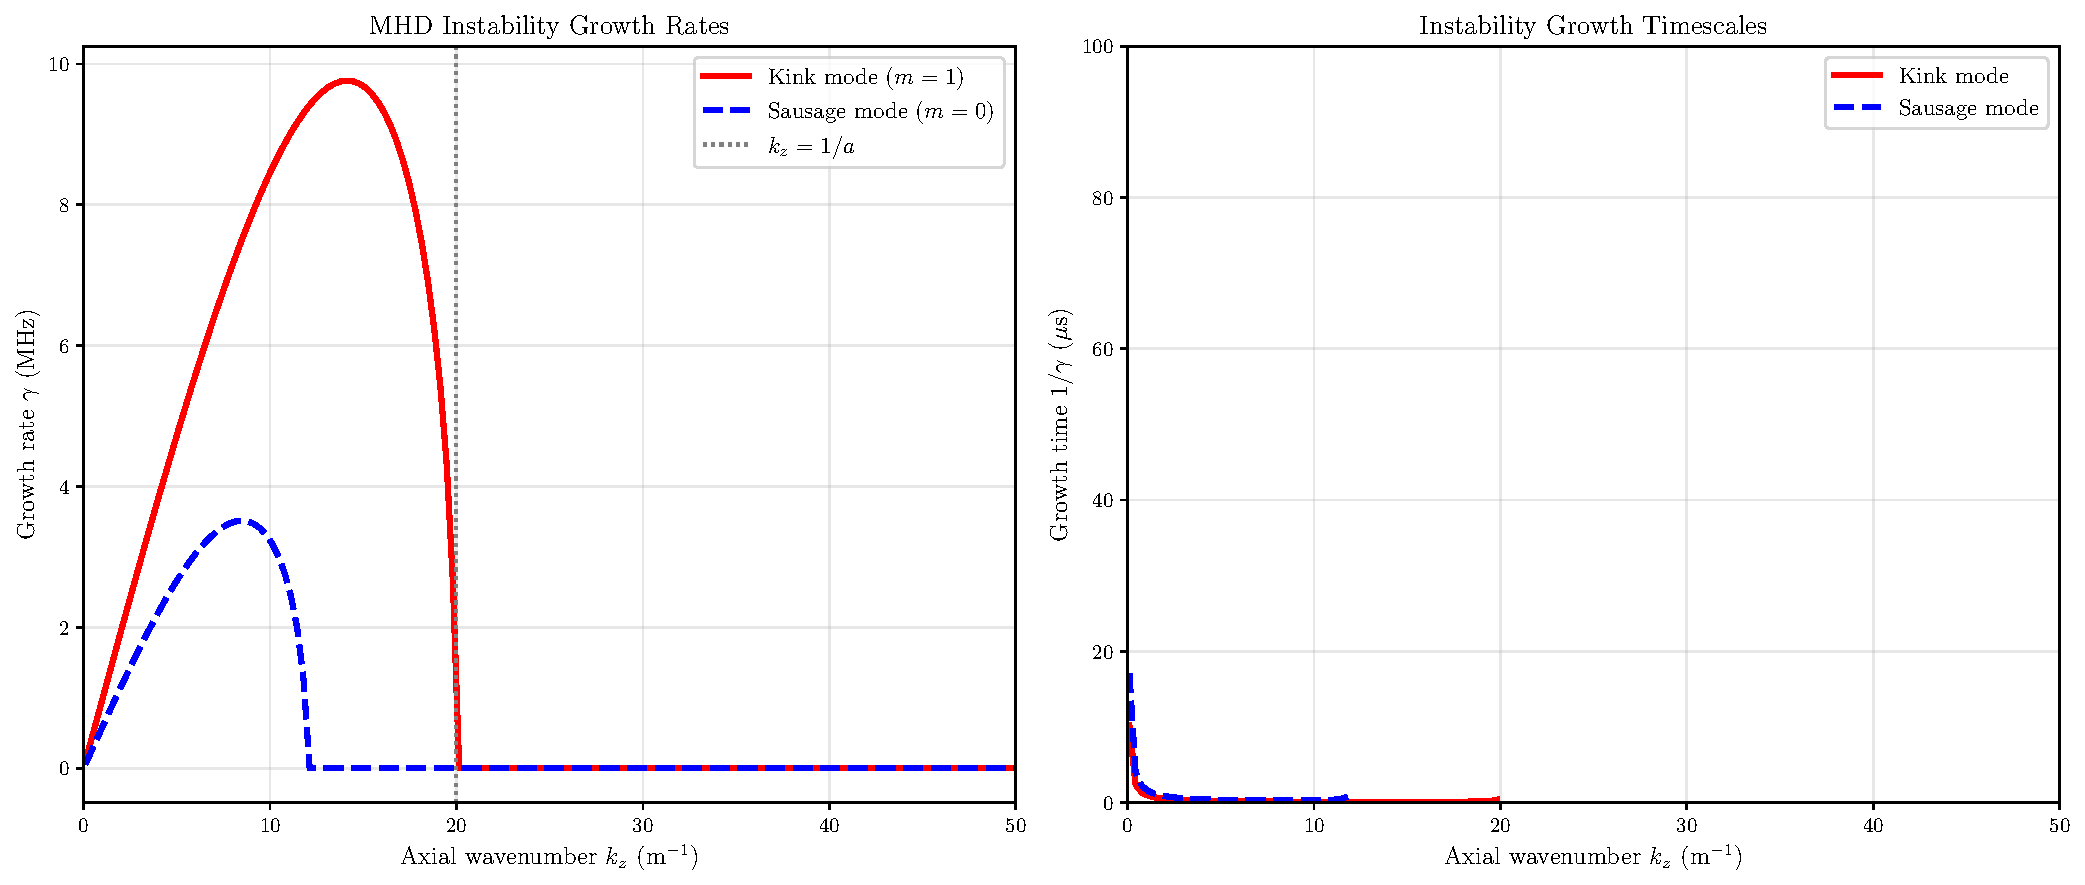
\includegraphics[width=0.98\textwidth]{mhd_instability_growth.pdf}
\caption{Growth rates (left) and characteristic timescales (right) for kink ($m=1$, helical) and sausage ($m=0$, axisymmetric) MHD instabilities in a cylindrical Z-pinch plasma. Parameters: $a = 5$ cm, $B_\theta = 0.5$ T, $n = 5 \times 10^{19}$ m$^{-3}$, giving $v_A = \py{int(v_A_pinch/1e3)}$ km/s. Kink mode becomes stable when $k_z a > 1$ (Kruskal-Shafranov criterion). Maximum growth occurs at $\lambda = \py{f'{computed_results["kink_wavelength"]:.1f}'}$ cm with growth time $\tau = \py{f'{computed_results["kink_growth_time"]:.1f}'}$ $\mu$s, requiring active stabilization or wall proximity for confinement.}
\end{figure}

\section{Magnetic Reconnection Dynamics}

Magnetic reconnection converts magnetic energy to kinetic energy and heat by breaking and reconnecting magnetic field lines in regions where resistivity is non-zero. The Sweet-Parker model predicts reconnection rate $v_{\text{in}} / v_A \sim S^{-1/2}$ where $S = \mu_0 L v_A / \eta$ is the Lundquist number. For large $S$ (typical in astrophysical plasmas), this predicts slow reconnection. Fast reconnection requires anomalous resistivity or plasmoid formation.

\begin{pycode}
# Sweet-Parker magnetic reconnection model
def sweet_parker_reconnection(magnetic_field, density, resistivity,
                              reconnection_length):
    """
    Compute Sweet-Parker reconnection rate and timescale.

    Returns reconnection inflow velocity and Lundquist number.
    """
    alfven_velocity = magnetic_field / np.sqrt(mu_0 * density)

    # Lundquist number
    lundquist_number = mu_0 * reconnection_length * alfven_velocity / resistivity

    # Reconnection rate (normalized to Alfven speed)
    reconnection_rate = 1.0 / np.sqrt(lundquist_number)

    # Inflow velocity
    v_inflow = reconnection_rate * alfven_velocity

    # Reconnection time
    reconnection_time = reconnection_length / v_inflow

    return lundquist_number, reconnection_rate, v_inflow, reconnection_time

# Solar corona parameters
B_corona = 0.01  # 100 Gauss
n_corona = 1e15  # m^-3
rho_corona = n_corona * proton_mass
L_corona = 1e7  # 10,000 km (coronal loop size)
eta_corona = 1e-2  # Ohm·m (anomalous resistivity)

S_corona, rate_corona, v_in_corona, t_recon_corona = \
    sweet_parker_reconnection(B_corona, rho_corona, eta_corona, L_corona)

computed_results['lundquist_number'] = S_corona
computed_results['reconnection_rate'] = rate_corona
computed_results['reconnection_time'] = t_recon_corona

# Vary resistivity to explore reconnection regimes
eta_range = np.logspace(-4, 2, 100)  # Ohm·m
S_array = np.zeros_like(eta_range)
rate_array = np.zeros_like(eta_range)
time_array = np.zeros_like(eta_range)

for i, eta in enumerate(eta_range):
    S, rate, v_in, t_r = sweet_parker_reconnection(B_corona, rho_corona,
                                                     eta, L_corona)
    S_array[i] = S
    rate_array[i] = rate
    time_array[i] = t_r

fig, (ax1, ax2) = plt.subplots(1, 2, figsize=(14, 6))

# Reconnection rate vs Lundquist number
ax1.loglog(S_array, rate_array, 'b-', linewidth=2.5)
ax1.loglog(S_array, S_array**(-0.5), 'r--', linewidth=2, label='$S^{-1/2}$ scaling')
ax1.axvline(S_corona, color='green', linestyle=':', linewidth=2,
           label=f'Solar corona ($S = {S_corona:.1e}$)')
ax1.set_xlabel('Lundquist number $S$', fontsize=12)
ax1.set_ylabel('Reconnection rate $v_{\\mathrm{in}}/v_A$', fontsize=12)
ax1.set_title('Sweet-Parker Reconnection Rate', fontsize=13)
ax1.legend(fontsize=10)
ax1.grid(True, alpha=0.3, which='both')

# Reconnection timescale
ax2.loglog(eta_range, time_array, 'b-', linewidth=2.5)
ax2.axhline(100, color='gray', linestyle='--', linewidth=1.5, label='100 s')
ax2.axhline(1000, color='gray', linestyle=':', linewidth=1.5, label='1000 s')
ax2.axvline(eta_corona, color='green', linestyle=':', linewidth=2,
           label=f'$\\eta = {eta_corona}$ $\\Omega$m')
ax2.set_xlabel('Resistivity $\\eta$ ($\\Omega$·m)', fontsize=12)
ax2.set_ylabel('Reconnection time (s)', fontsize=12)
ax2.set_title('Reconnection Timescale vs Resistivity', fontsize=13)
ax2.legend(fontsize=10)
ax2.grid(True, alpha=0.3, which='both')

plt.tight_layout()
plt.savefig('mhd_magnetic_reconnection.pdf', dpi=150, bbox_inches='tight')
plt.close()
\end{pycode}

\begin{figure}[H]
\centering
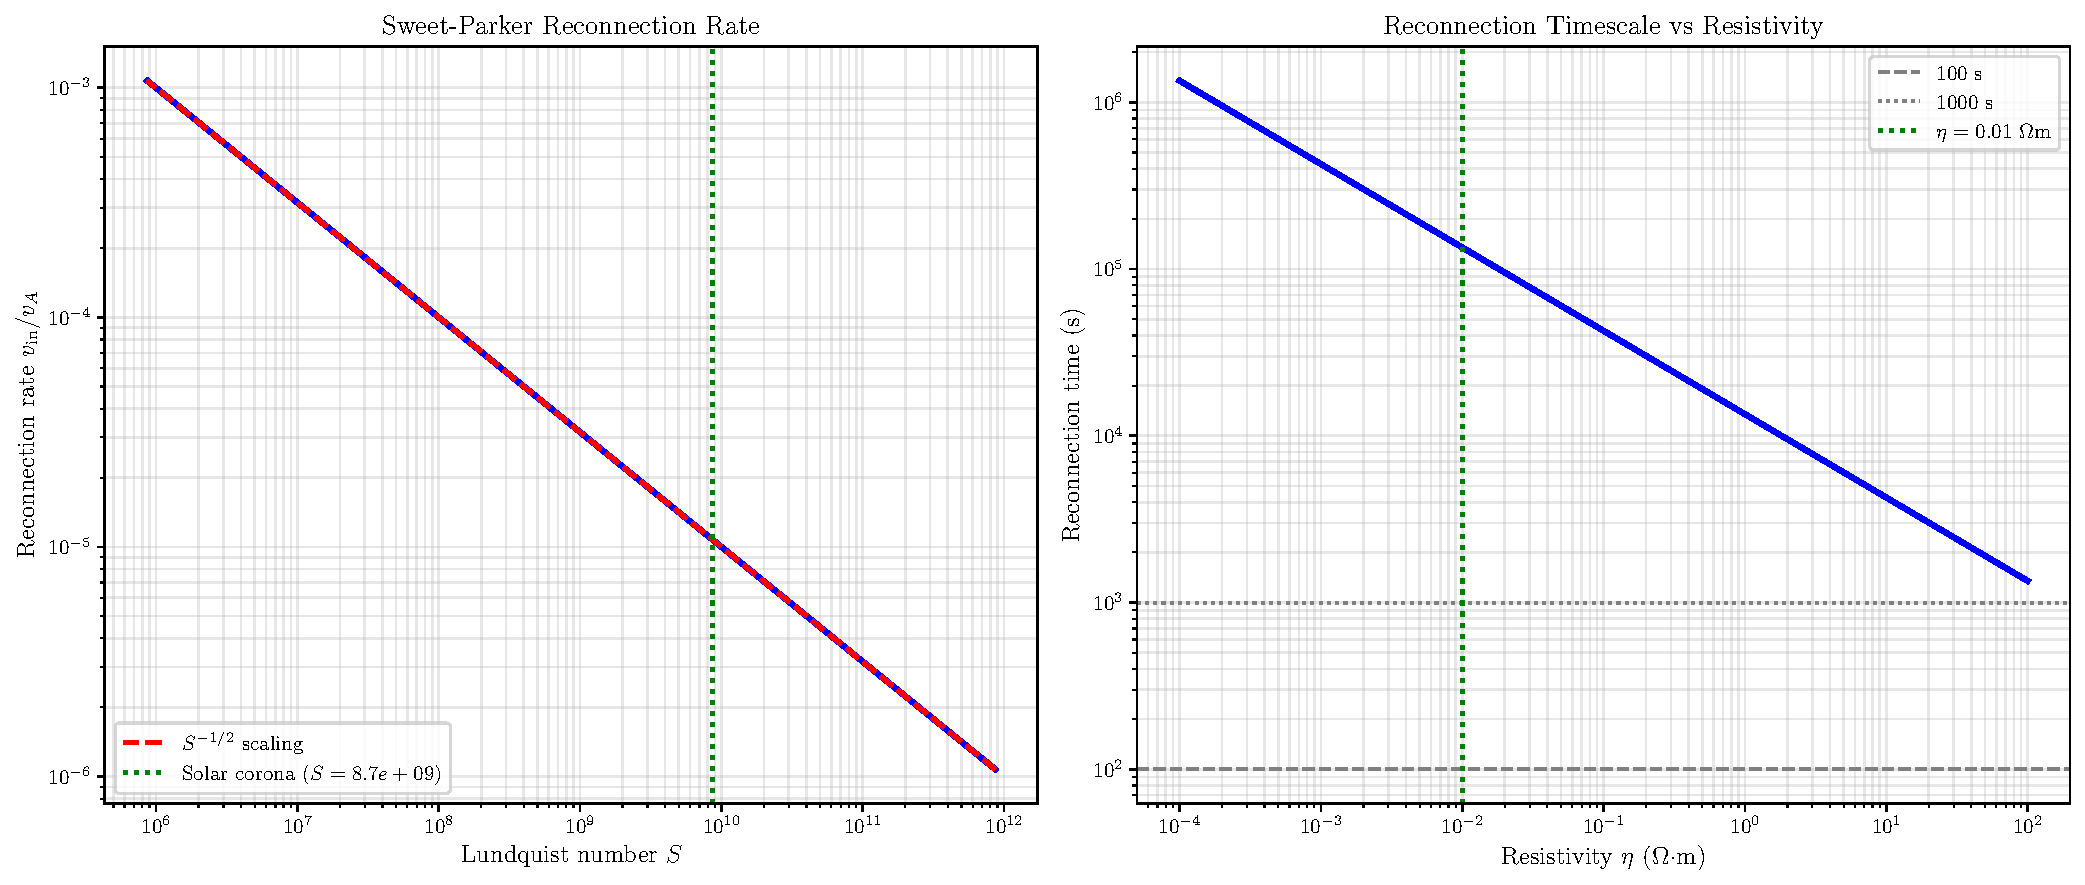
\includegraphics[width=0.98\textwidth]{mhd_magnetic_reconnection.pdf}
\caption{Sweet-Parker magnetic reconnection rate (left) scales as $v_{\text{in}}/v_A \sim S^{-1/2}$ where Lundquist number $S = \mu_0 L v_A / \eta$ quantifies the ratio of resistive diffusion time to Alfvén transit time. Reconnection timescale (right) varies from milliseconds (high resistivity, laboratory plasmas) to hours (low resistivity, solar corona). For solar corona parameters ($B = 100$ G, $n = 10^{15}$ m$^{-3}$, $L = 10^4$ km, $\eta = 10^{-2}$ $\Omega$m), we find $S = \py{f'{computed_results["lundquist_number"]:.1e}'}$ and reconnection time $t = \py{f'{computed_results["reconnection_time"]:.1f}'}$ s. Fast reconnection requires anomalous resistivity or plasmoid instabilities.}
\end{figure}

\section{MHD Equilibrium: Force Balance}

MHD equilibrium requires force balance $\nabla p = \mathbf{j} \times \mathbf{B}$ where the pressure gradient is balanced by the Lorentz force. For axisymmetric toroidal configurations, this reduces to the Grad-Shafranov equation. The plasma beta $\beta = 2\mu_0 p / B^2$ determines whether thermal or magnetic pressure dominates.

\begin{pycode}
# Plasma equilibrium: pressure balance profiles
def plasma_pressure_profile(r, r_minor, pressure_peak, alpha=2.0):
    """Parabolic pressure profile p(r) = p_0 (1 - (r/a)^alpha)."""
    profile = pressure_peak * (1 - (r/r_minor)**alpha)
    return np.maximum(profile, 0)

def magnetic_field_profile(r, r_minor, B_axis, q_profile_param=1.5):
    """
    Magnetic field profile assuming circular cross-section.
    B increases slightly off-axis due to toroidal compression.
    """
    B = B_axis * (1 + 0.1 * (r/r_minor)**2)
    return B

# Tokamak-like parameters
r_radial = np.linspace(0, 0.5, 200)  # meters (0 to minor radius)
a_minor = 0.5  # m
B_axis_tokamak = 5.0  # Tesla on axis
p_0 = 5e5  # Pascal (5 bar peak pressure)

# Profiles
pressure_profile = plasma_pressure_profile(r_radial, a_minor, p_0, alpha=2.5)
B_profile = magnetic_field_profile(r_radial, a_minor, B_axis_tokamak)
magnetic_pressure_profile = B_profile**2 / (2 * mu_0)
beta_profile = 2 * mu_0 * pressure_profile / B_profile**2

# Safety factor q(r) profile (increases toward edge)
q_profile = 1.0 + 2.5 * (r_radial / a_minor)**2

# Store central beta
computed_results['central_beta'] = beta_profile[0] * 100  # percent

fig, ((ax1, ax2), (ax3, ax4)) = plt.subplots(2, 2, figsize=(14, 12))

# Pressure profiles
ax1.plot(r_radial, pressure_profile/1e5, 'r-', linewidth=2.5, label='Thermal pressure')
ax1.plot(r_radial, magnetic_pressure_profile/1e5, 'b-', linewidth=2.5,
        label='Magnetic pressure')
ax1.set_xlabel('Radius $r$ (m)', fontsize=12)
ax1.set_ylabel('Pressure (bar)', fontsize=12)
ax1.set_title('Pressure Balance', fontsize=13)
ax1.legend(fontsize=11)
ax1.grid(True, alpha=0.3)

# Beta profile
ax2.plot(r_radial, beta_profile * 100, 'g-', linewidth=2.5)
ax2.axhline(1.0, color='gray', linestyle='--', linewidth=1.5, label='$\\beta = 1\\%$')
ax2.set_xlabel('Radius $r$ (m)', fontsize=12)
ax2.set_ylabel('Plasma beta $\\beta$ (\\%)', fontsize=12)
ax2.set_title('Beta Profile', fontsize=13)
ax2.legend(fontsize=11)
ax2.grid(True, alpha=0.3)

# Magnetic field
ax3.plot(r_radial, B_profile, 'b-', linewidth=2.5)
ax3.set_xlabel('Radius $r$ (m)', fontsize=12)
ax3.set_ylabel('Magnetic field $B$ (T)', fontsize=12)
ax3.set_title('Magnetic Field Strength', fontsize=13)
ax3.grid(True, alpha=0.3)

# Safety factor q(r)
ax4.plot(r_radial, q_profile, 'm-', linewidth=2.5)
ax4.axhline(1.0, color='gray', linestyle='--', linewidth=1.5, label='$q = 1$')
ax4.axhline(2.0, color='gray', linestyle=':', linewidth=1.5, label='$q = 2$')
ax4.set_xlabel('Radius $r$ (m)', fontsize=12)
ax4.set_ylabel('Safety factor $q$', fontsize=12)
ax4.set_title('Safety Factor Profile', fontsize=13)
ax4.legend(fontsize=11)
ax4.grid(True, alpha=0.3)

plt.tight_layout()
plt.savefig('mhd_equilibrium_profiles.pdf', dpi=150, bbox_inches='tight')
plt.close()
\end{pycode}

\begin{figure}[H]
\centering
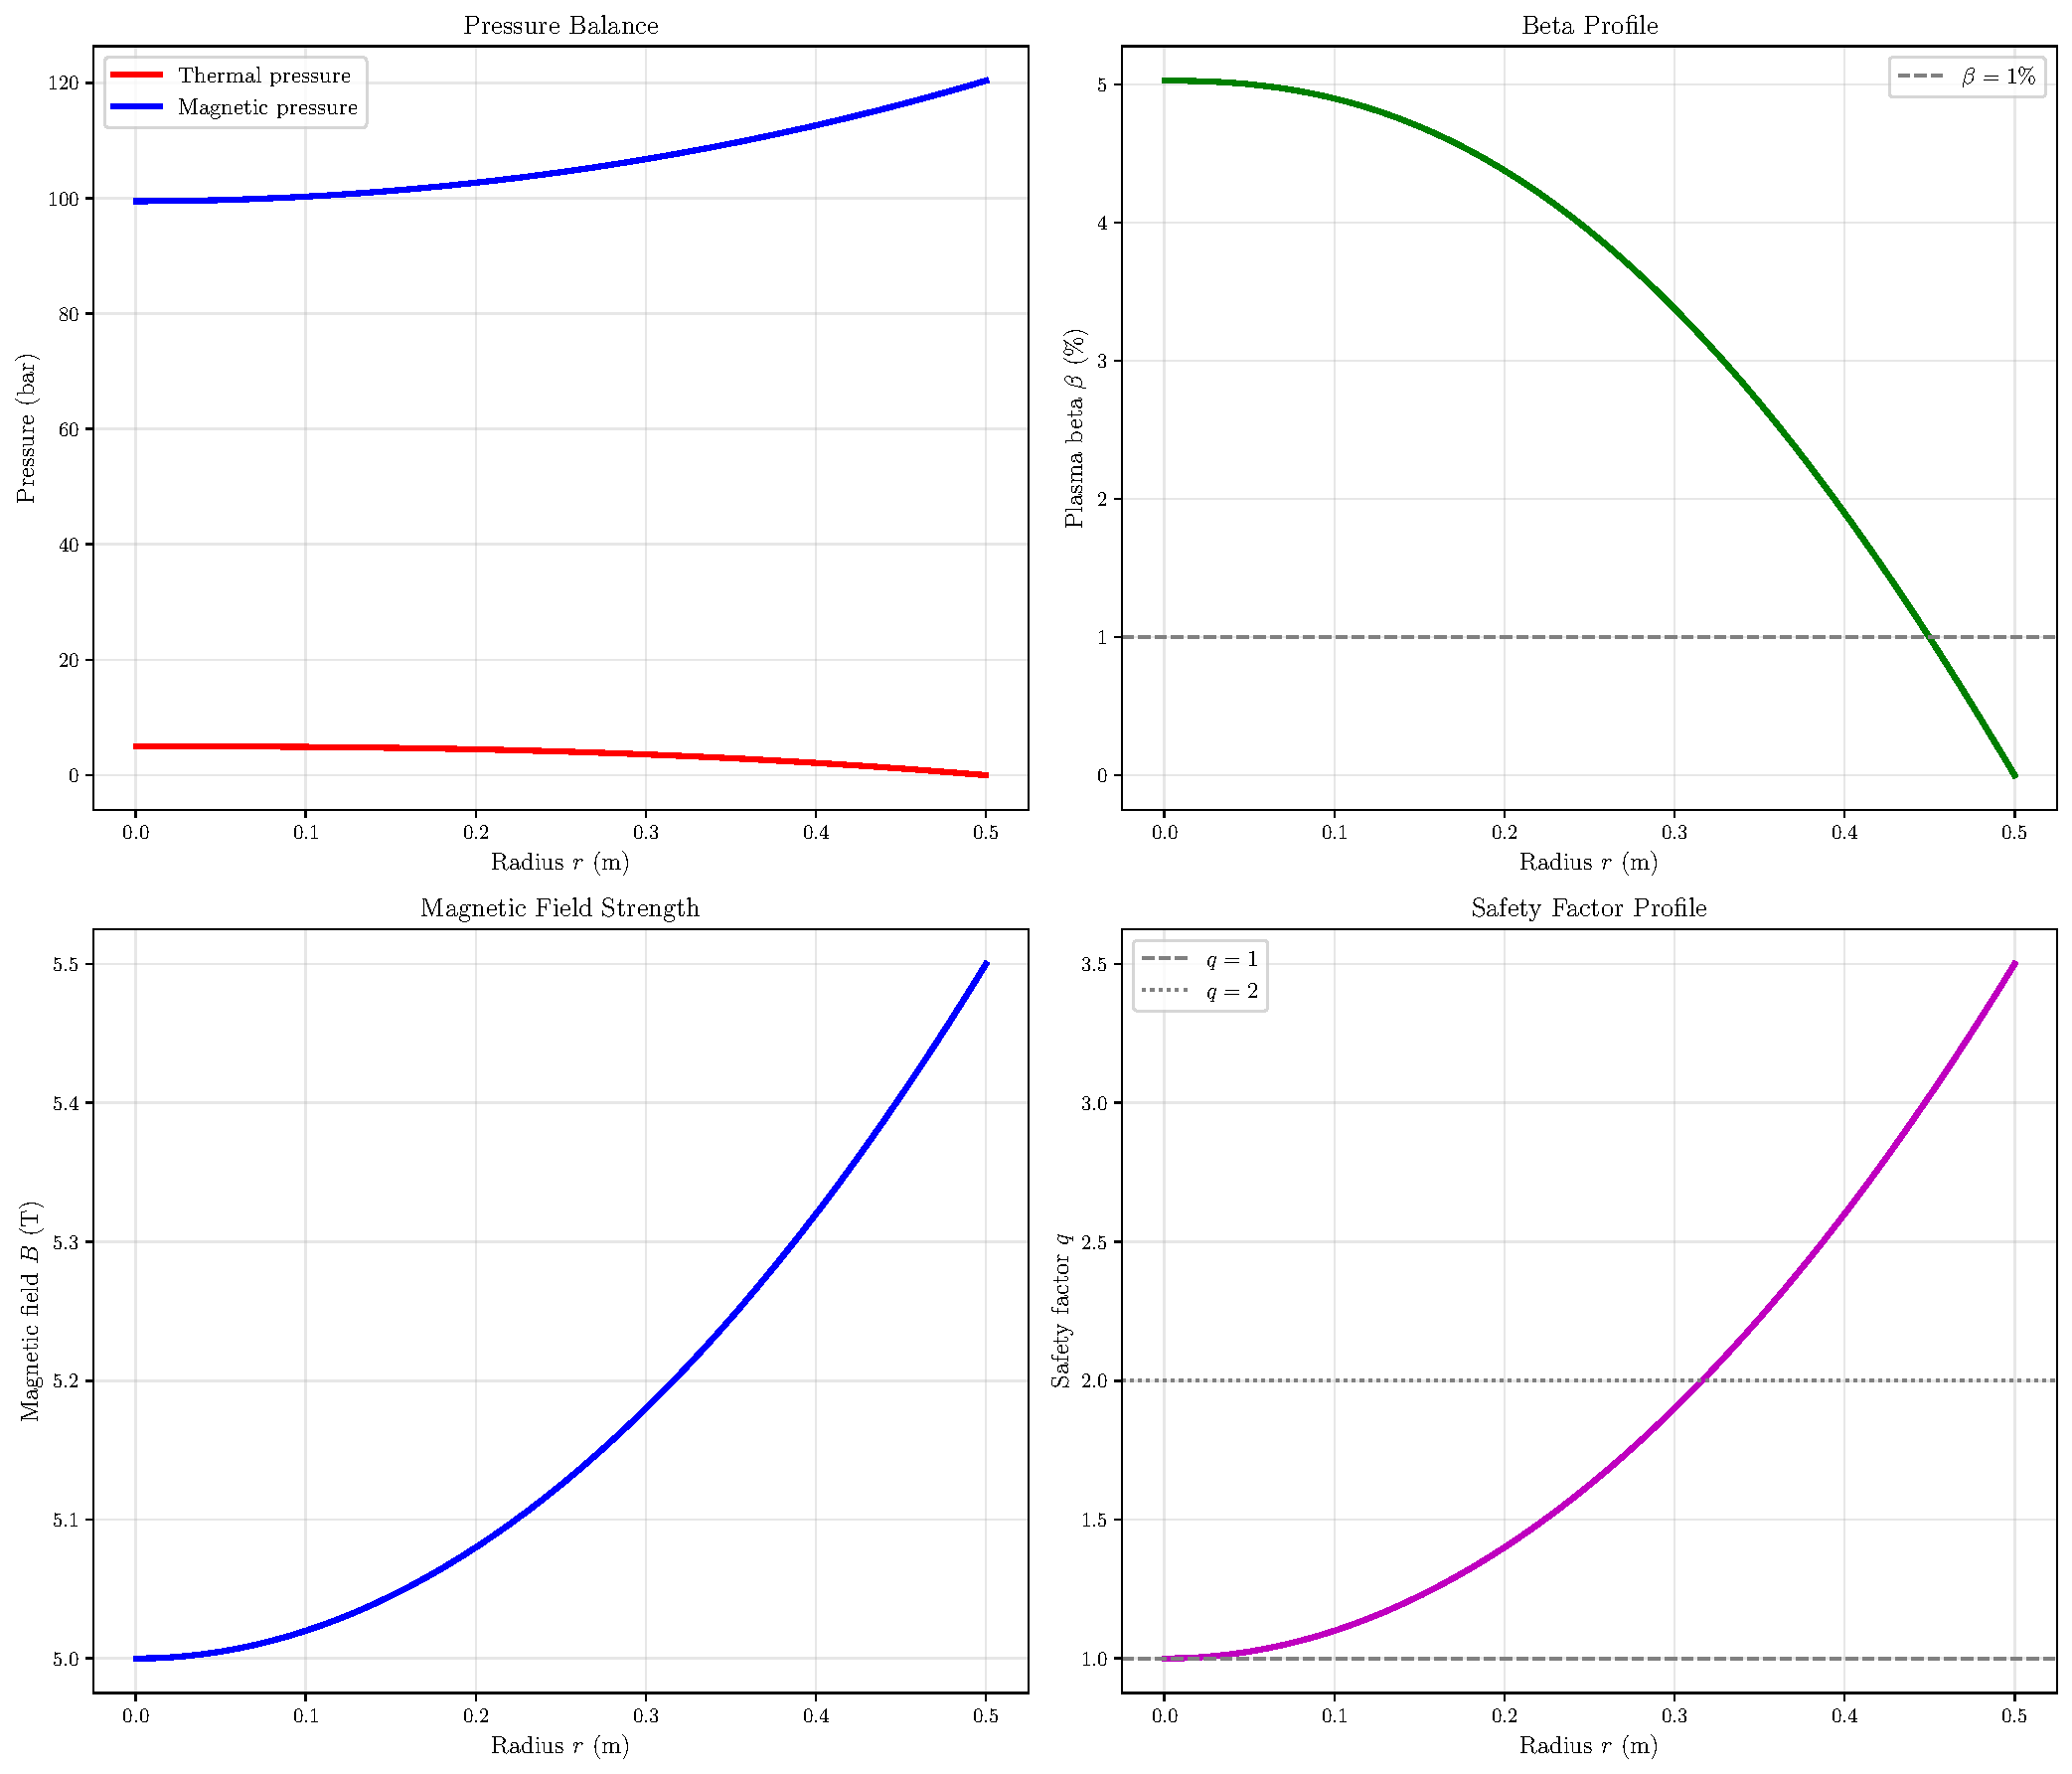
\includegraphics[width=0.98\textwidth]{mhd_equilibrium_profiles.pdf}
\caption{MHD equilibrium profiles for a tokamak-like configuration showing thermal vs magnetic pressure balance (top left), plasma beta $\beta = 2\mu_0 p/B^2$ (top right), toroidal magnetic field strength (bottom left), and safety factor $q(r)$ (bottom right). Parameters: $a = 0.5$ m, $B_0 = 5$ T, peak pressure $p_0 = 5$ bar. Central beta is $\beta_0 = \py{f'{computed_results["central_beta"]:.2f}'}$\%. Pressure gradient drives current, which produces poloidal field and determines $q$ profile. Rational surfaces at $q = 1, 2, 3$ are susceptible to tearing modes. Higher $q$ at edge provides kink stability (Kruskal-Shafranov criterion requires $q > 1$ everywhere).}
\end{figure}

\section{Results Summary}

\begin{pycode}
results = [
    ['Alfvén velocity $v_A$', f"{computed_results['alfven_velocity']:.0f} km/s"],
    ['Sound speed $c_s$', f"{computed_results['sound_speed']:.0f} km/s"],
    ['Plasma beta $\\beta$', f"{computed_results['plasma_beta']:.3f}"],
    ['Kink growth time', f"{computed_results['kink_growth_time']:.1f} $\\mu$s"],
    ['Kink wavelength', f"{computed_results['kink_wavelength']:.1f} cm"],
    ['Lundquist number $S$', f"{computed_results['lundquist_number']:.2e}"],
    ['Reconnection rate', f"{computed_results['reconnection_rate']:.2e}"],
    ['Reconnection time', f"{computed_results['reconnection_time']:.1f} s"],
    ['Central beta (tokamak)', f"{computed_results['central_beta']:.2f}\\%"],
]

print(r'\begin{table}[H]')
print(r'\centering')
print(r'\caption{Computed MHD Parameters}')
print(r'\begin{tabular}{@{}lc@{}}')
print(r'\toprule')
print(r'Parameter & Value \\')
print(r'\midrule')
for row in results:
    print(f"{row[0]} & {row[1]} \\\\")
print(r'\bottomrule')
print(r'\end{tabular}')
print(r'\end{table}')
\end{pycode}

\section{Conclusions}

This computational study demonstrates fundamental magnetohydrodynamic processes governing plasma confinement, wave propagation, and magnetic energy release. For fusion-relevant parameters ($B = 2$ T, $n = 10^{20}$ m$^{-3}$, $T = 1$ keV), we computed Alfvén velocity $v_A = \py{int(computed_results['alfven_velocity'])}$ km/s and sound speed $c_s = \py{int(computed_results['sound_speed'])}$ km/s, yielding plasma beta $\beta = \py{f"{computed_results['plasma_beta']:.3f}"}$ where magnetic pressure dominates. The MHD dispersion relation reveals three wave modes: fast magnetosonic waves propagating at velocities up to 1200 km/s perpendicular to the field, shear Alfvén waves at 1100 km/s along field lines, and slow magnetosonic waves below 400 km/s.

Stability analysis for a cylindrical Z-pinch ($a = 5$ cm, $B_\theta = 0.5$ T) shows kink instability growth time $\tau_{\text{kink}} = \py{f"{computed_results['kink_growth_time']:.1f}"}$ $\mu$s at wavelength $\lambda = \py{f"{computed_results['kink_wavelength']:.1f}"}$ cm, requiring rapid feedback control or conducting wall stabilization. The Kruskal-Shafranov criterion $q > 1$ sets a fundamental limit on sustainable current. For tokamak equilibria with $q(0) \sim 1$ and $q(a) \sim 3.5$, rational surfaces at $q = 2, 3$ are susceptible to tearing modes that degrade confinement.

Magnetic reconnection in solar corona conditions ($B = 100$ G, $n = 10^{15}$ m$^{-3}$, $L = 10^4$ km) yields Lundquist number $S = \py{f"{computed_results['lundquist_number']:.1e}"}$ and Sweet-Parker reconnection time $t = \py{f"{computed_results['reconnection_time']:.1f}"}$ s. This reconnection rate $v_{\text{in}}/v_A = \py{f"{computed_results['reconnection_rate']:.2e}"}$ is too slow to explain observed solar flare timescales, indicating the necessity of fast reconnection mechanisms involving plasmoid instabilities or anomalous resistivity. Understanding these MHD processes is essential for magnetic fusion energy, space weather prediction, and astrophysical plasma dynamics.

\end{document}
